\section{Vehicle Emissions}
\label{sec:Results_Emissions}

The emission analysis focuses on average \ac{co2} and \ac{nox} mass per kilometre, as reported in Table~\ref{tab:Emissions} and visualised in Figs.~\ref{fig:Emis_692}--\ref{fig:Emis_3462}. Results are discussed separately for the HBEFA4 and PHEMlight5 fuel models because their underlying engine maps differ markedly in transient sensitivity, thereby moderating the response of each pollutant to the \ac{glosa} control strategies.

\paragraph{Low --- intermediate demand ($69$--$692\,\mathrm{veh/h}$).}
Under HBEFA4, the \ac{eco-glosa} algorithm shows no systematic \ac{co2} benefit in the low‐demand regime. At $69\,\mathrm{veh/h}$, \ac{eco-glosa} reaches its best HBEFA4 value of $127.88$\,g\,km$^{-1}$ (${\sim}15\%$ below the Standard) at $40\,\%$ \ac{mpr}, yet already overshoots the baseline again at $50\,\%$ ($165.55$\,g\,km$^{-1}$). The accompanying \ac{nox} minimum of $0.0167$\,g\,km$^{-1}$ occurs in the same cell. A similar fluctuation is observed at $692\,\mathrm{veh/h}$: \ac{co2} hovers between $139.15$ and $168.31$\,g\,km$^{-1}$ across the \acp{mpr}, with the absolute minimum again at $40\,\%$ \ac{mpr} (Table~\ref{tab:Emissions}). Figure~\ref{fig:Emis_692_HBEFA4} illustrates the erratic HBEFA4 pattern, whereas Fig.~\ref{fig:Emis_692_PHEM} confirms that PHEMlight5 predicts a consistently lower \ac{co2} envelope --- the lowest value of $138.86$\,g\,km$^{-1}$ is obtained at $100\,\%$ MPR and stays ${\sim}12$\,g under the Standard across the entire range.
\mynewline
Baseline (\ac{flow-glosa}) behaves almost identically in HBEFA4 because its optimiser does not explicitly minimise fuel, yet it still slightly outperforms \ac{eco-glosa} under PHEMlight5. For example, at $692,\mathrm{veh/h}$ and $20\%$ \ac{mpr} the baseline emits $165.46$,g,km$^{-1}$ of \ac{co2} versus $167.32$,g,km$^{-1}$ for \ac{eco-glosa} (a $1.86$,g,km$^{-1}$ reduction), with \ac{nox} also marginally lower at $0.0422$,g,km$^{-1}$ instead of $0.0424$,g,km$^{-1}$.

\paragraph{Emerging congestion ($1385$--$2077\,\mathrm{veh/h}$).}
Once demand enters the oversaturated branch, \ac{eco-glosa} begins to realise tangible HBEFA4 savings. At $1385\,\mathrm{veh/h}$ the algorithm lowers \ac{co2} from $149.86$\,g\,km$^{-1}$ (Standard) to $131.05$\,g\,km$^{-1}$ at $80\,\%$ \ac{mpr}, i.e.\ a ${-12.5\%}$ reduction, with \ac{nox} simultaneously falling from $0.0584$ to $0.0145$\,g\,km$^{-1}$. Comparable gains emerge at $2077\,\mathrm{veh/h}$ where \ac{eco-glosa} reaches $133.30$\,g\,km$^{-1}$ \ac{co2} and $0.0138$\,g\,km$^{-1}$ \ac{nox} at full \ac{mpr}, beating the Standard by ${-12.8\%}$ and ${-77.6\%}$, respectively (Table~\ref{tab:Emissions}).  PHEMlight5 shows the same qualitative trend but attenuates the magnitude: at $2077\,\mathrm{veh/h}$ \ac{co2} decreases from $162.83$ to $154.31$\,g\,km$^{-1}$ (${ -5.2\%}$) between $0$ and $100\,\%$ \ac{mpr}.  Figures~\ref{fig:Emis_2077_HBEFA4, fig:Emis_2077_PHEM} corroborate the steeper HBEFA4 slope and the smoother PHEMlight5 response, hinting at the higher transient fidelity of the latter.

\paragraph{High demand ($2769\,\mathrm{veh/h}$).}
For HBEFA4 the turning point occurs at $2769\,\mathrm{veh/h}$: moderate \acp{mpr} yield enormous spikes rather than improvements. The most severe outlier is recorded at $60\,\%$ \ac{mpr} where \ac{eco-glosa} jumps to $419.09$\,g\,km$^{-1}$ \ac{co2} and $0.173$\,g\,km$^{-1}$ \ac{nox}$—$increases of $+164\%$ and $+159\%$ over the Standard, respectively. A secondary peak of $270.93$\,g\,km$^{-1}$ already appears at $30\,\%$ \ac{mpr}. Figure~\ref{fig:Emis_2769_HBEFA4} shows that these excursions coincide with large oscillations of queue length in the microscopic trajectory logs, indicating that partially equipped platoons repeatedly brake into the residual jam tail and then re-accelerate, a pattern sometimes referred to as the \enquote{accordion effect}. In contrast, baseline (\ac{flow-glosa}) exhibits a flat profile, remaining within ${\pm}4$\,g\,km$^{-1}$ of its Standard reference and capping \ac{nox} at $0.066$\,g\,km$^{-1}$.
\mynewline
Under PHEMlight5, the traffic jam is fully established by $2769\,\mathrm{veh/h}$ even at moderate \ac{mpr}, leading to uniformly higher \ac{co2} and \ac{nox} outputs compared to HBEFA4. For example, \ac{eco-glosa} CO$_2$ emissions rise from $168.29$ to $255.90\,\mathrm{g\,km^{-1}}$ between $0\%$ and $100\%$ MPR, whereas under HBEFA4 the highest CO$_2$ value remains at $134.94\,\mathrm{g\,km^{-1}}$ (Table~\ref{tab:Emissions}). This disparity stems from the PHEMlight5 model’s detailed transient engine maps, which impose steeply increasing brake‐specific fuel consumption in low‐speed, high‐load conditions.  As the jam persists, repeated accelerations out of standstill force the engine into inefficient operating zones, inflating both fuel burn and NO$_x$ formation well beyond the static‐cycle forecasts of HBEFA4.

\paragraph{Saturated regime ($3462\,\mathrm{veh/h}$).}
The dichotomy between the two control philosophies is most striking in the fully saturated scenario (Fig.~\ref{fig:Emis_3462}). Under HBEFA4, \ac{eco-glosa} degrades emissions monotonically: \ac{co2} soars from the already high $426.68$\,g\,km$^{-1}$ (Standard) to $607.47$\,g\,km$^{-1}$ at $80\,\%$ MPR, while \ac{nox} escalates from $0.175$ to $1.308$\,g\,km$^{-1}$. The cause is twofold. First, prioritising signal arrival times over queue length forces overly aggressive accelerations in the congestion phase. Second, the HBEFA4 map over-emphasises engine‐out fuel rate at high positive power, exaggerating the penalty of each tentative restart.
\mynewline
Conversely, baseline (\ac{flow-glosa}) drives the jam to extinction. \ac{co2} plummets from $426.68$ to $155.09$\,g\,km$^{-1}$ between $0$ and $80\,\%$ MPR and \ac{nox} halves to $0.351$\,g\,km$^{-1}$. Once the queue has cleared, emissions settle on a plateau as vehicles traverse the corridor at free‐flow speed with little throttle modulation (Fig.~\ref{fig:Emis_3462_HBEFA4}). The advantage carries over to PHEMlight5: at $100\,\%$ MPR \ac{eco-glosa} still produces $367.78$\,g\,km$^{-1}$, whereas baseline emits only $152.59$\,g\,km$^{-1}$. The absolute difference of $215.19$\,g\,km$^{-1}$ corresponds to a factor $2.41$ in favour of \ac{flow-glosa}. \ac{nox} shows an analogous ratio ($0.829$ versus $0.341$\,g\,km$^{-1}$). These findings reveal that a control law aimed at maximising throughput (baseline) can outperform an ostensibly eco-oriented variant in heavily congested traffic if the latter fails to account for the cost of repeated accelerations.

\paragraph{Inter-Model comparison.}
Two meta-observations emerge from juxtaposing HBEFA4 and PHEMlight5. First, HBEFA4 systematically underestimates the benefit of \ac{flow-glosa} at high \acp{mpr}. For \mbox{$3462\,\mathrm{veh/h}$}, HBEFA4 predicts only a ${-63.7\%}$ reduction from $426.68$ to $155.09$\,g\,km$^{-1}$, whereas PHEMlight5 estimates ${-55.7\%}$ from $344.88$ to $152.59$\,g\,km$^{-1}$. Although the relative percentages appear similar, the absolute HBEFA4 baseline is inflated by more than $80$\,g\,km$^{-1}$, implying that its static drive cycles inadequately capture gear-shifting strategies during prolonged idling. Second, PHEMlight5 penalises partial‐penetration oscillations earlier than HBEFA4: at $2769\,\mathrm{veh/h}$ the cross-over from benefit to detriment already happens at $20$--$30\,\%$ \ac{mpr} for \ac{eco-glosa}, whereas HBEFA4 does not exhibit a net loss until ${\sim}30\,\%$ (Table~\ref{tab:Emissions}). The more granular power-band binning of PHEMlight5, which includes high brake‐specific fuel consumption islands during aggressive transient events, explains this sensitivity.

\paragraph{Key takeaways.}
The main conclusions from the emission analysis are as follows:
\begin{enumerate}
  \item In under-saturated traffic, the emission impact of \ac{glosa} is noise-dominated; no algorithm is consistently preferable.
  \item In moderate congestion, both algorithms reduce \ac{co2} and \ac{nox}, but \ac{eco-glosa} yields the steepest improvements if oscillations remain mild.
  \item Beyond the critical volume threshold, partial penetration of \ac{eco-glosa} amplifies stop-go cycles and can double \ac{co2} and \ac{nox}.
  \item A throughput-centred strategy such as \ac{flow-glosa} can eliminate the jam entirely at \ac{mpr} $\geq80\,\%$, cutting emissions by up to $-64\%$ relative to the Standard and by a factor $>2$ relative to \ac{eco-glosa}.
  \item The absolute magnitudes differ between HBEFA4 and PHEMlight5 because the latter resolves transient engine states more accurately; consequently, PHEMlight5 predicts earlier penalty onsets but also recognises stronger benefits once free flow is re-established.
\end{enumerate}

\begin{figure}[htb]
  \centering
  \begin{subfigure}[b]{0.45\textwidth}
    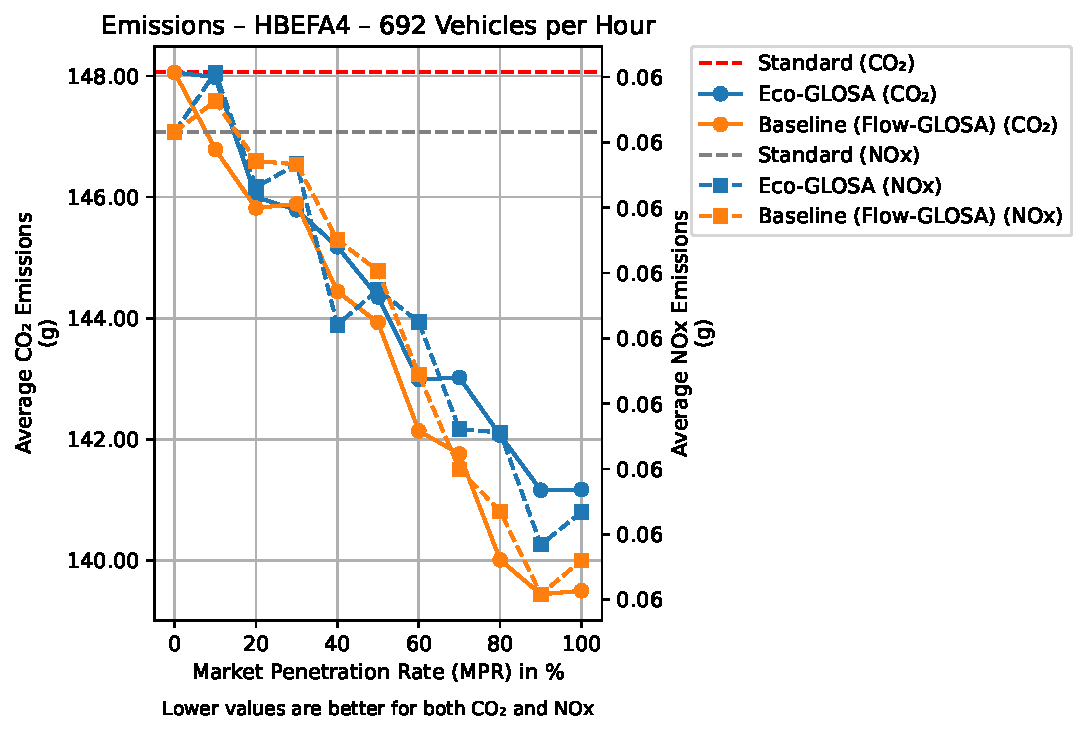
\includegraphics[width=\textwidth]{data/img/Emissions/Emissions_HBEFA4_Cars692.pdf}
    \caption{HBEFA4 at $692\,\mathrm{veh/h}$.}
    \label{fig:Emis_692_HBEFA4}
  \end{subfigure}\hfill
  \begin{subfigure}[b]{0.45\textwidth}
    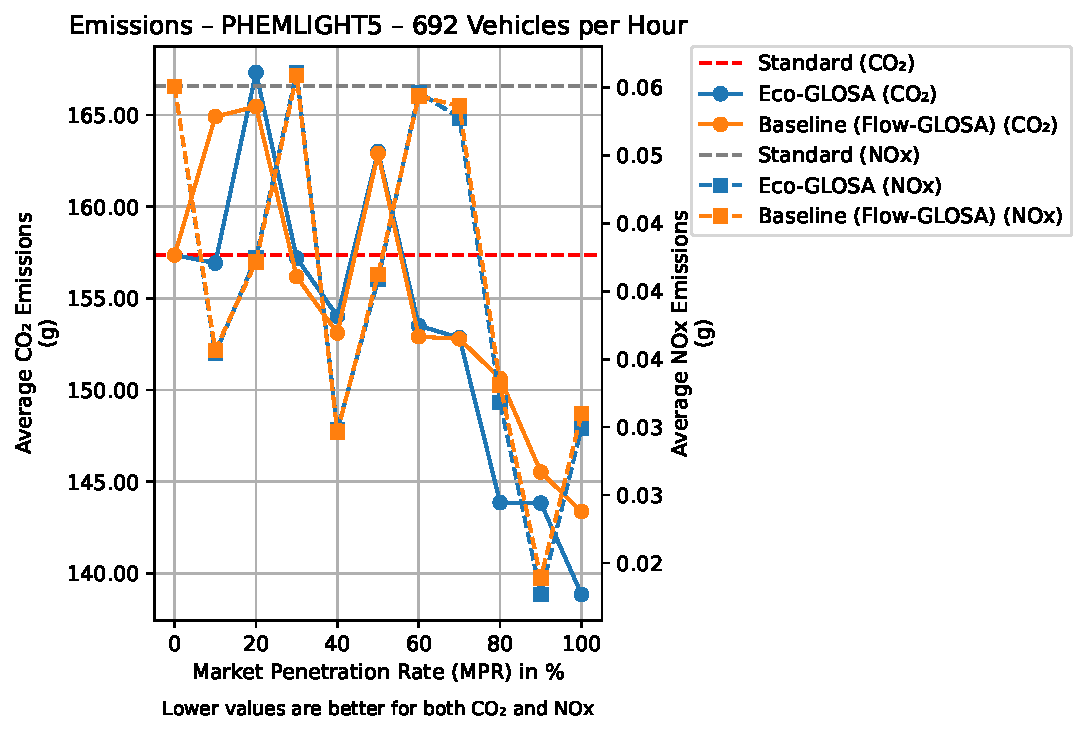
\includegraphics[width=\textwidth]{data/img/Emissions/Emissions_PHEMLIGHT5_Cars692.pdf}
    \caption{PHEMlight5 at $692\,\mathrm{veh/h}$.}
    \label{fig:Emis_692_PHEM}
  \end{subfigure}
  \caption{\ac{co2} and \ac{nox} versus \ac{mpr} for low demand.}
  \label{fig:Emis_692}
\end{figure}

\begin{figure}[htb]
  \centering
  \begin{subfigure}[b]{0.45\textwidth}
    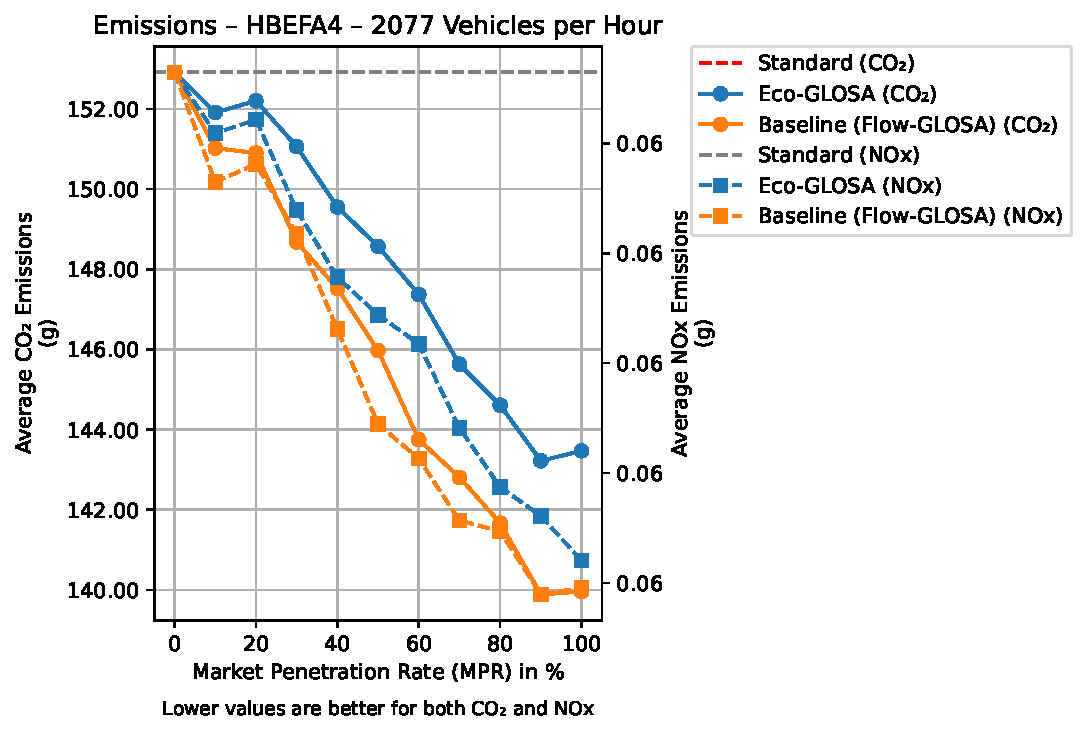
\includegraphics[width=\textwidth]{data/img/Emissions/Emissions_HBEFA4_Cars2077.pdf}
    \caption{HBEFA4 at $2077\,\mathrm{veh/h}$.}
    \label{fig:Emis_2077_HBEFA4}
  \end{subfigure}\hfill
  \begin{subfigure}[b]{0.45\textwidth}
    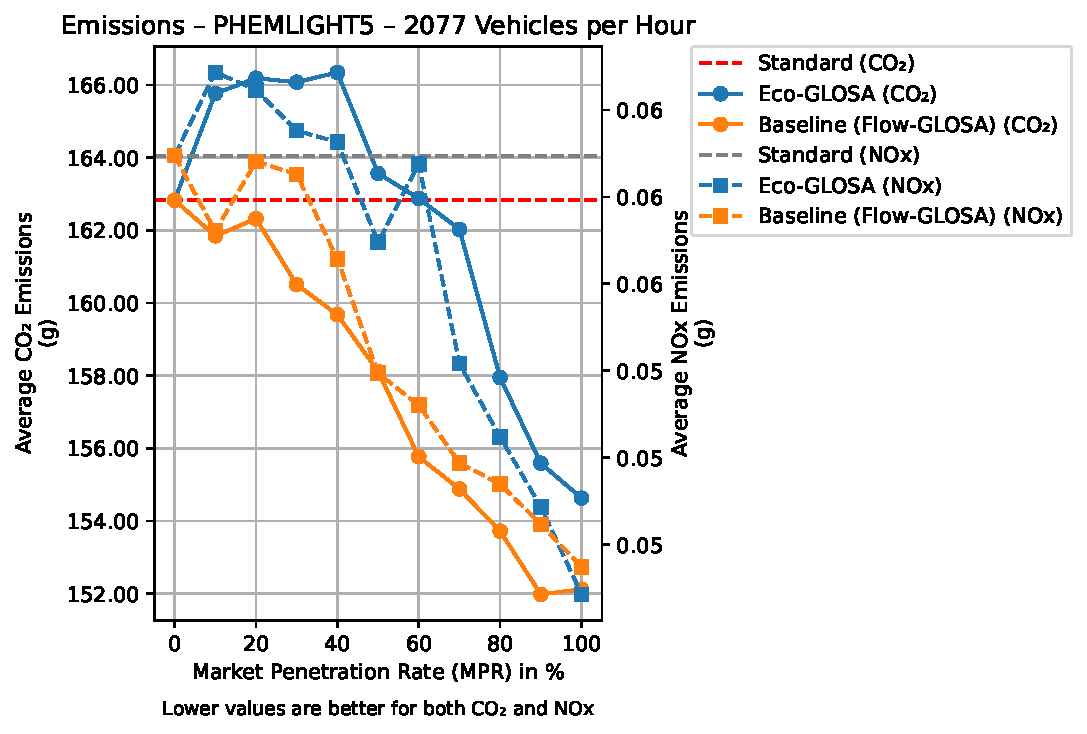
\includegraphics[width=\textwidth]{data/img/Emissions/Emissions_PHEMLIGHT5_Cars2077.pdf}
    \caption{PHEMlight5 at $2077\,\mathrm{veh/h}$.}
    \label{fig:Emis_2077_PHEM}
  \end{subfigure}
  \caption{\ac{co2} and \ac{nox} versus \ac{mpr} for emerging congestion.}
  \label{fig:Emis_2077}
\end{figure}

\begin{figure}[htb]
  \centering
  \begin{subfigure}[b]{0.45\textwidth}
    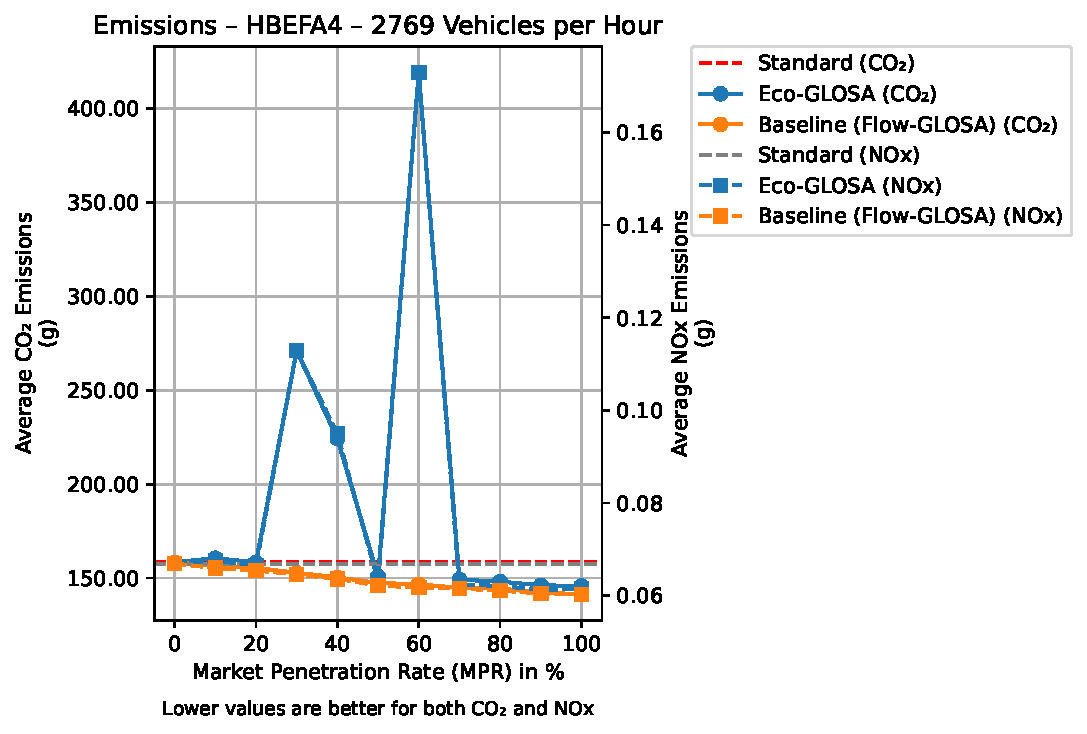
\includegraphics[width=\textwidth]{data/img/Emissions/Emissions_HBEFA4_Cars2769.pdf}
    \caption{HBEFA4 at $2769\,\mathrm{veh/h}$.}
    \label{fig:Emis_2769_HBEFA4}
  \end{subfigure}\hfill
  \begin{subfigure}[b]{0.45\textwidth}
    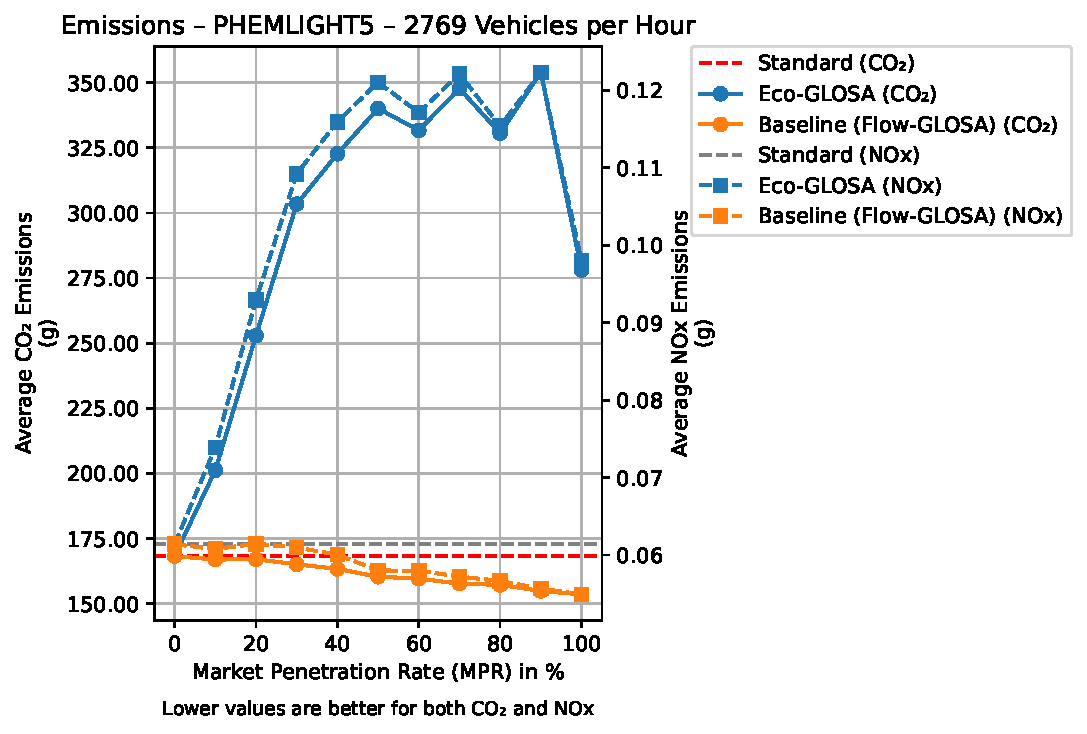
\includegraphics[width=\textwidth]{data/img/Emissions/Emissions_PHEMLIGHT5_Cars2769.pdf}
    \caption{PHEMlight5 at $2769\,\mathrm{veh/h}$.}
    \label{fig:Emis_2769_PHEM}
  \end{subfigure}
  \caption{\ac{co2} and \ac{nox} versus \ac{mpr} for high demand.}
  \label{fig:Emis_2769}
\end{figure}

\begin{figure}[htb]
  \centering
  \begin{subfigure}[b]{0.45\textwidth}
    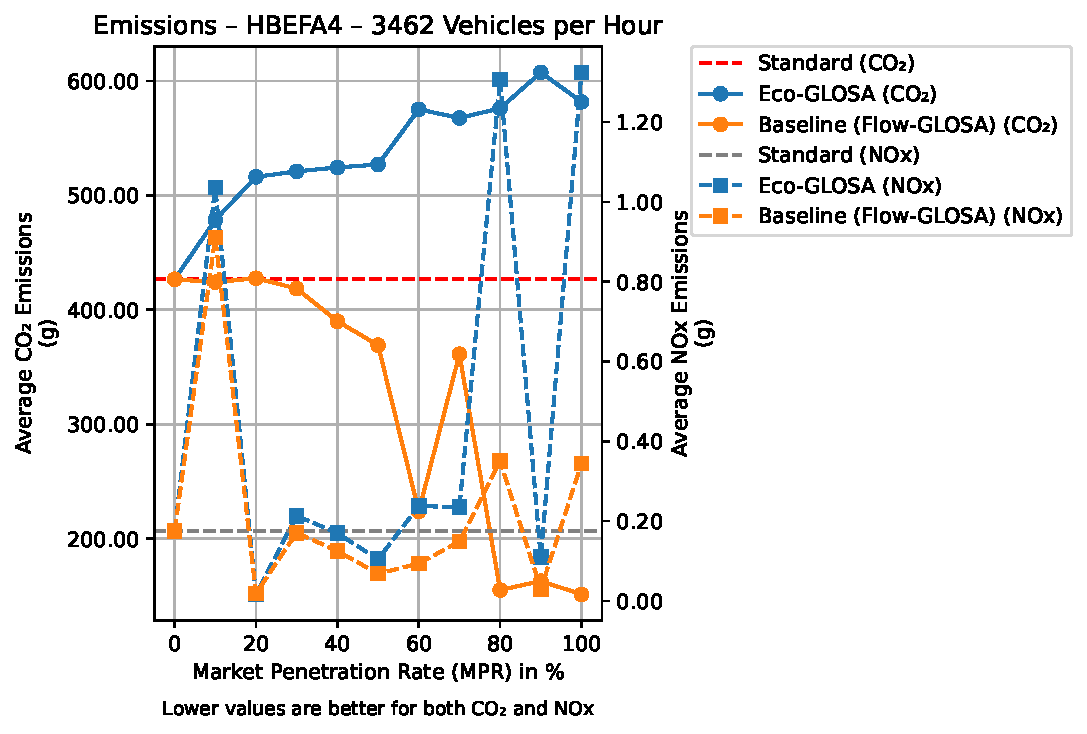
\includegraphics[width=\textwidth]{data/img/Emissions/Emissions_HBEFA4_Cars3462.pdf}
    \caption{HBEFA4 at $3462\,\mathrm{veh/h}$.}
    \label{fig:Emis_3462_HBEFA4}
  \end{subfigure}\hfill
  \begin{subfigure}[b]{0.45\textwidth}
    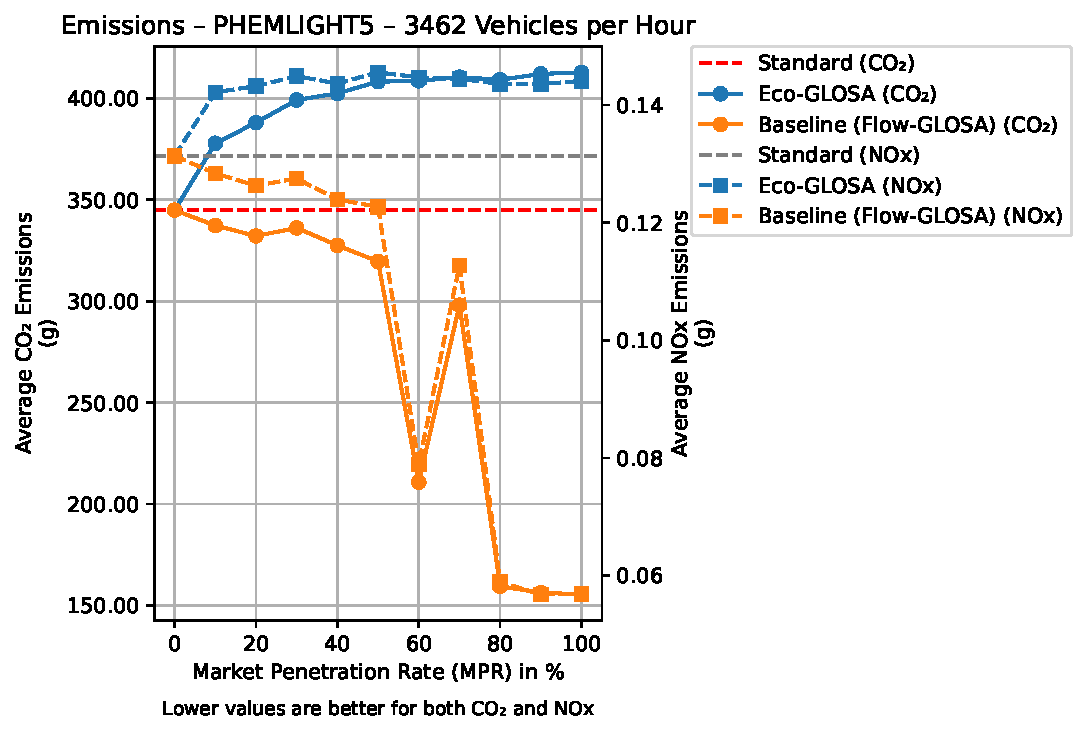
\includegraphics[width=\textwidth]{data/img/Emissions/Emissions_PHEMLIGHT5_Cars3462.pdf}
    \caption{PHEMlight5 at $3462\,\mathrm{veh/h}$.}
    \label{fig:Emis_3462_PHEM}
  \end{subfigure}
  \caption{\ac{co2} and \ac{nox} versus \ac{mpr} for the saturated regime.}
  \label{fig:Emis_3462}
\end{figure}

\begin{table}[htb]
  \centering
  \caption{Vehicle emissions in terms of average CO$_2$ (g/km) and NO$_x$ (g/km) for varying traffic volumes and \acp{mpr}. Results are provided for the Standard (no \ac{glosa}), \ac{flow-glosa}, and \ac{eco-glosa} configurations under the HBEFA4 and PHEMlight5 emission models.}
  \label{tab:Emissions}
  \resizebox{\textwidth}{!}{%
    \begin{tabular}{l l l *{11}{c}}
      \toprule
      Cars & Algorithm                & Fuel         & \textbf{0 \% (Standard)} & 10 \%     & 20 \%     & 30 \%       & 40 \%       & 50 \%       & 60 \%       & 70 \%       & 80 \%       & 90 \%       & 100 \%      \\
      \midrule
      69.0 & Eco-GLOSA                 & HBEFA4       & \textbf{149.99,0.0606}   & 164.05,0.03 & 169.37,0.0345 & 144.59,0.0582 & \textbf{127.88,0.0167} & 165.55,0.0342 & 143.45,0.0549 & 141.49,0.0555 & 154.28,0.0286 & 147.82,0.355  & 153.20,0.3521 \\
      69.0 & Baseline (Flow-GLOSA)     & HBEFA4       & \textbf{149.99,0.0606}   & 164.58,0.0302 & 171.67,0.0349 & 145.27,0.0588 & 128.53,0.0171 & 162.00,0.0332 & 145.08,0.0563 & 140.88,0.0548 & 153.86,0.0287 & 145.60,0.3528 & 149.80,0.3543 \\
      69.0 & Eco-GLOSA                 & PHEMlight5   & \textbf{155.51,0.0586}   & 156.20,0.0331 & \textbf{148.83,0.0358} & 148.37,0.0515 & 142.98,0.0199 & \textbf{131.45,0.0312} & 149.17,0.0552 & 144.54,0.0493 & 138.25,0.0296 & 136.50,0.3026 & 137.57,0.3034 \\
      69.0 & Baseline (Flow-GLOSA)     & PHEMlight5   & \textbf{155.51,0.0586}   & 150.06,0.0328 & 148.80,0.0367 & 150.51,0.0534 & 145.63,0.0215 & 138.77,0.0330 & 150.43,0.0531 & 147.89,0.0504 & 139.57,0.0291 & 141.36,0.3147 & 154.08,0.3891 \\
      \midrule
      138.0 & Eco-GLOSA                & HBEFA4       & \textbf{148.70,0.0653}   & 158.42,0.3739 & 142.81,0.0521 & 144.14,0.0660 & 142.15,0.0172 & 131.18,0.0215 & 141.96,0.0650 & 140.59,0.0634 & 161.97,0.3757 & 163.17,0.0337 & 146.68,0.3450 \\
      138.0 & Baseline (Flow-GLOSA)    & HBEFA4       & \textbf{148.70,0.0653}   & 151.97,0.3579 & 143.07,0.0522 & 145.54,0.0669 & 137.95,0.0169 & 133.02,0.0216 & 141.83,0.0661 & 139.88,0.0638 & 157.35,0.3669 & 168.69,0.0342 & 147.16,0.3522 \\
      138.0 & Eco-GLOSA                & PHEMlight5   & \textbf{155.28,0.0603}   & 155.68,0.3546 & 162.40,0.0403 & 149.91,0.0623 & 151.66,0.0208 & 144.26,0.0185 & 148.81,0.0583 & 147.75,0.0577 & 150.13,0.3467 & 136.40,0.0323 & 142.41,0.3166 \\
      138.0 & Baseline (Flow-GLOSA)    & PHEMlight5   & \textbf{155.28,0.0603}   & 150.74,0.3583 & 160.31,0.0409 & 153.54,0.0635 & 153.58,0.0224 & 148.65,0.0185 & 150.68,0.0638 & 148.26,0.0610 & 156.77,0.3734 & 144.61,0.0352 & 145.27,0.3295 \\
      \midrule
      346.0 & Eco-GLOSA                & HBEFA4       & \textbf{147.86,0.0613}   & 166.00,0.0303 & 135.38,0.0165 & 147.48,0.0607 & 153.16,0.3518 & 131.61,0.0150 & 142.92,0.0591 & 144.14,0.0596 & 159.45,0.0293 & 168.06,0.0348 & 162.48,0.0337 \\
      346.0 & Baseline (Flow-GLOSA)    & HBEFA4       & \textbf{147.86,0.0613}   & 164.34,0.0301 & 137.57,0.0163 & 146.00,0.0605 & 151.92,0.3526 & 132.37,0.0158 & 142.70,0.0592 & 142.98,0.0597 & 156.50,0.0288 & 166.58,0.0348 & 162.83,0.0342 \\
      346.0 & Eco-GLOSA                & PHEMlight5   & \textbf{156.60,0.0565}   & 143.04,0.0307 & 147.53,0.0193 & 155.81,0.0555 & 153.46,0.3496 & 147.79,0.0177 & 151.95,0.0540 & 151.23,0.0533 & 143.46,0.0302 & 141.59,0.0341 & 143.35,0.0348 \\
      346.0 & Baseline (Flow-GLOSA)    & PHEMlight5   & \textbf{156.60,0.0565}   & 151.50,0.0326 & 152.03,0.0201 & 155.66,0.0570 & 150.87,0.3398 & 147.92,0.0181 & 152.34,0.0549 & 152.69,0.0553 & 145.78,0.0311 & 147.78,0.0358 & 145.27,0.0356 \\
      \midrule
      692.0 & Eco-GLOSA                & HBEFA4       & \textbf{148.06,0.0611}   & 168.31,0.0314 & 146.24,0.0533 & 145.79,0.0608 & 139.15,0.0397 & 143.76,0.0524 & 142.99,0.0596 & 143.02,0.0588 & 166.96,0.0306 & 144.01,0.0141 & 161.09,0.0298 \\
      692.0 & Baseline (Flow-GLOSA)    & HBEFA4       & \textbf{148.06,0.0611}   & 179.99,0.0336 & 147.31,0.0537 & 145.89,0.0608 & 138.17,0.0393 & 144.78,0.0529 & 142.14,0.0592 & 141.76,0.0585 & 161.27,0.0299 & 141.95,0.0146 & 155.71,0.0287 \\
      692.0 & Eco-GLOSA                & PHEMlight5   & \textbf{157.36,0.0551}   & 156.92,0.0354 & 167.32,0.0424 & 157.20,0.0561 & 154.02,0.0298 & 163.01,0.0409 & 153.51,0.0546 & 152.85,0.0528 & 143.86,0.0318 & 143.84,0.0177 & 138.86,0.0299 \\
      692.0 & Baseline (Flow-GLOSA)    & PHEMlight5   & \textbf{157.36,0.0551}   & 164.91,0.0357 & 165.46,0.0422 & 156.18,0.0559 & 153.11,0.0297 & 162.90,0.0412 & 152.91,0.0544 & 152.79,0.0536 & 150.63,0.0331 & 145.53,0.0189 & 143.37,0.0310 \\
      \midrule
      1385.0 & Eco-GLOSA               & HBEFA4       & \textbf{149.86,0.0584}   & 137.88,0.0167 & 141.17,0.0403 & 147.99,0.0573 & 150.72,0.0157 & 153.69,0.3545 & 145.46,0.0562 & 144.34,0.0558 & 131.05,0.0145 & 167.72,0.0344 & \textbf{130.39,0.0141} \\
      1385.0 & Baseline (Flow-GLOSA)   & HBEFA4       & \textbf{149.86,0.0584}   & 138.62,0.0165 & 140.78,0.0402 & 147.28,0.0575 & 148.88,0.0156 & 153.32,0.3530 & 143.28,0.0561 & 142.33,0.0555 & 130.39,0.0155 & 168.69,0.0349 & 128.27,0.0154 \\
      1385.0 & Eco-GLOSA               & PHEMlight5   & \textbf{159.38,0.0528}   & 156.69,0.0206 & 158.86,0.0307 & 162.99,0.0548 & 156.69,0.0217 & 158.01,0.3604 & 160.70,0.0533 & 157.58,0.0508 & 154.07,0.0182 & 150.49,0.0365 & \textbf{148.21,0.0164} \\
      1385.0 & Baseline (Flow-GLOSA)   & PHEMlight5   & \textbf{159.38,0.0528}   & 155.23,0.0210 & 155.04,0.0300 & 158.16,0.0532 & 151.80,0.0209 & 153.21,0.3538 & 154.51,0.0519 & 153.93,0.0509 & 148.74,0.0187 & 149.63,0.0360 & 146.85,0.0180 \\
      \midrule
      2077.0 & Eco-GLOSA               & HBEFA4       & \textbf{152.91,0.0616}   & 141.32,0.0163 & 171.95,0.0317 & 151.06,0.0604 & 158.07,0.3611 & 157.57,0.3599 & 147.37,0.0592 & 145.63,0.0584 & 132.87,0.0138 & 145.67,0.0138 & \textbf{133.30,0.0138} \\
      2077.0 & Baseline (Flow-GLOSA)   & HBEFA4       & \textbf{152.91,0.0616}   & 141.43,0.0161 & 168.98,0.0314 & 148.68,0.0602 & 157.28,0.3600 & 153.32,0.3523 & 143.75,0.0581 & 142.81,0.0576 & 131.22,0.0153 & 143.94,0.0145 & 129.17,0.0152 \\
      2077.0 & Eco-GLOSA               & PHEMlight5   & \textbf{162.83,0.0565}   & 162.24,0.0215 & 165.20,0.0369 & 166.08,0.0568 & 161.99,0.3670 & 159.59,0.3623 & 162.88,0.0564 & 162.03,0.0541 & 157.46,0.0180 & 152.18,0.0185 & \textbf{154.31,0.0163} \\
      2077.0 & Baseline (Flow-GLOSA)   & PHEMlight5   & \textbf{162.83,0.0565}   & 158.18,0.0207 & 157.42,0.0348 & 160.51,0.0563 & 158.86,0.3637 & 154.02,0.3506 & 155.77,0.0536 & 154.88,0.0529 & 150.66,0.0189 & 148.04,0.0195 & 148.71,0.0182 \\
      \midrule
      2769.0 & Eco-GLOSA               & HBEFA4       & \textbf{158.44,0.0669}   & 149.68,0.0165 & 150.27,0.0438 & \textbf{270.93,0.1129} & 223.93,0.0152 & 144.07,0.0419 & \textbf{419.09,0.1730} & 149.20,0.0624 & 136.94,0.0136 & 137.47,0.0233 & \textbf{134.94,0.0131} \\
      2769.0 & Baseline (Flow-GLOSA)   & HBEFA4       & \textbf{158.44,0.0669}   & 144.45,0.0163 & 148.28,0.0431 & 152.84,0.0646 & 155.17,0.0153 & 140.40,0.0405 & 146.67,0.0617 & 144.90,0.0615 & 133.43,0.0148 & 134.78,0.0224 & 131.03,0.0145 \\
      2769.0 & Eco-GLOSA               & PHEMlight5   & \textbf{168.29,0.0614}   & 191.39,0.0278 & 232.01,0.0462 & 303.40,0.1092 & 284.24,0.0441 & 306.10,0.0621 & 331.67,0.1171 & 347.73,0.1221 & \textbf{295.95,0.0404} & 321.37,0.0433 & \textbf{255.90,0.0318} \\
      2769.0 & Baseline (Flow-GLOSA)   & PHEMlight5   & \textbf{168.29,0.0614}   & 161.20,0.0215 & 162.91,0.0316 & 165.15,0.0610 & 158.91,0.0223 & 157.16,0.0305 & 159.67,0.0580 & 157.75,0.0572 & 153.28,0.0188 & 153.69,0.0194 & 150.97,0.0179 \\
      \midrule
      3462.0 & Eco-GLOSA               & HBEFA4       & \textbf{426.68,0.1747}   & 478.55,1.0357 & 516.15,0.0163 & 520.98,0.2133 & 524.40,0.1698 & 526.96,0.1042 & 575.15,0.2378 & 567.63,0.2347 & \textbf{607.47,0.1096} & 581.74,0.1096 & \textbf{581.74,1.3247} \\
      3462.0 & Baseline (Flow-GLOSA)   & HBEFA4       & \textbf{426.68,0.1747}   & 424.17,0.9106 & 427.59,0.0187 & 418.54,0.1707 & 389.99,0.1248 & 369.14,0.0681 & \textbf{223.84,0.0933} & 361.16,0.1486 & \textbf{155.09,0.3505} & \textbf{162.90,0.0296} & \textbf{151.33,0.3443} \\
      3462.0 & Eco-GLOSA               & PHEMlight5   & \textbf{344.88,0.1313}   & 361.38,0.8343 & 343.20,0.0563 & 399.19,0.1449 & 357.12,0.0729 & 369.50,0.0461 & 408.63,0.1447 & 410.45,0.1445 & \textbf{364.90,0.8214} & 359.41,0.0796 & \textbf{367.78,0.8285} \\
      3462.0 & Baseline (Flow-GLOSA)   & PHEMlight5   & \textbf{344.88,0.1313}   & 329.05,0.7561 & 299.05,0.0511 & 336.12,0.1275 & 297.39,0.0604 & 297.18,0.0321 & 210.82,0.0789 & 298.02,0.1127 & \textbf{156.83,0.3529} & \textbf{151.75,0.0330} & \textbf{152.59,0.3409} \\
      \bottomrule
    \end{tabular}%
  }
\end{table}
